% begin module transformations-magnifications
\begin{frame}
\begin{columns}[c]
\column{.5\textwidth}

\psset{xunit=0.7cm, yunit=0.7cm}
\begin{pspicture}(-4, -3.5)(4.5,5)
\tiny
\fcAxesStandard{-4}{-3.5}{4.5}{5}
%Function formula: 10/3+1/3 ((-3+3 (x))^{3})-1/3 ((-3+3 (x))^{2})-1/3 (x)
\only<handout:1| 1->{
\psplot[linecolor=red, plotpoints=1000]{1.65}{2.55}{x -0.333333 mul x 3 mul -6 add 2 exp -0.333333 mul x 3 mul -6 add 3 exp 0.333333 mul 2.66667 add add add }
\rput[b] (2.55, 2.40654){$y=f(x)$}
}
%\only<handout:0| 3->{
%\psplot[linecolor=blue, plotpoints=1000]{1.65}{2.55}{x -0.333333 mul x 3 mul %-6 add 2 exp -0.333333 mul x 3 mul -6 add 3 exp 0.333333 mul 2.66667 add add %add }
%\rput[b] (2.55, 2.40654){$y=f(x)$}
%}

\only<handout:0| 3>{
\psplot[linecolor=red, plotpoints=1000]{1.65}{2.55}{x -0.333333 mul x 3 mul -6 add 2 exp -0.333333 mul x 3 mul -6 add 3 exp 0.333333 mul 2.66667 add add add 2 mul}
\rput[b] (2.55, 4.80654){{$y=cf(x)$}}
}
\only<handout:1| 4->{
\psplot[linecolor=blue, plotpoints=1000]{1.65}{2.55}{x -0.333333 mul x 3 mul -6 add 2 exp -0.333333 mul x 3 mul -6 add 3 exp 0.333333 mul 2.66667 add add add 2 mul}
\rput[b] (2.55, 4.80654){$y=cf(x)$}
}

\only<handout:0| 4>{
\psplot[linecolor=red, plotpoints=1000]{1.65}{2.55}{x -0.333333 mul x 3 mul -6 add 2 exp -0.333333 mul x 3 mul -6 add 3 exp 0.333333 mul 2.66667 add add add 2 div}
\rput[b] (2.55, 0.40654){{$y=\frac{1}{c}f(x)$}}
}
\only<handout:1| 5->{
\psplot[linecolor=blue, plotpoints=1000]{1.65}{2.55}{x -0.333333 mul x 3 mul -6 add 2 exp -0.333333 mul x 3 mul -6 add 3 exp 0.333333 mul 2.66667 add add add 2 div}
\rput[b] (2.55, 0.40654){$y=\frac{1}{c}f(x)$}
}

\only<handout:0| 5>{
\psplot[linecolor=red, plotpoints=1000]{1.65}{2.55}{x -0.333333 mul x 3 mul -6 add 2 exp -0.333333 mul x 3 mul -6 add 3 exp 0.333333 mul 2.66667 add add add -1 mul}
\rput[t] (2.55, -2.40654){{$y=-f(x)$}}
}
\only<handout:1| 6->{
\psplot[linecolor=blue, plotpoints=1000]{1.65}{2.55}{x -0.333333 mul x 3 mul -6 add 2 exp -0.333333 mul x 3 mul -6 add 3 exp 0.333333 mul 2.66667 add add add -1 mul}
\rput[t] (2.55, -2.40654){$y=-f(x)$}
}

\only<handout:0| 6>{
%Function formula: 8/3+1/3 ((-6-3 (x))^{3})+1/3 (x)-1/3 ((-6-3 (x))^{2})
\psplot[linecolor=red, plotpoints=1000]{-2.55}{-1.65}{x -3 mul -6 add 2 exp -0.333333 mul x 0.333333 mul x -3 mul -6 add 3 exp 0.333333 mul 2.66667 add add add }
\rput[b] (-2.55, 2.40654){{$y=f(-x)$}}
}
\only<handout:1| 7->{
%Function formula: 8/3+1/3 ((-6-3 (x))^{3})+1/3 (x)-1/3 ((-6-3 (x))^{2})
\psplot[linecolor=blue, plotpoints=1000]{-2.55}{-1.65}{x -3 mul -6 add 2 exp -0.333333 mul x 0.333333 mul x -3 mul -6 add 3 exp 0.333333 mul 2.66667 add add add }
\rput[b] (-2.55, 2.40654){$y=f(-x)$}
}
\end{pspicture}
%\ \only<handout:0| -2>{%
%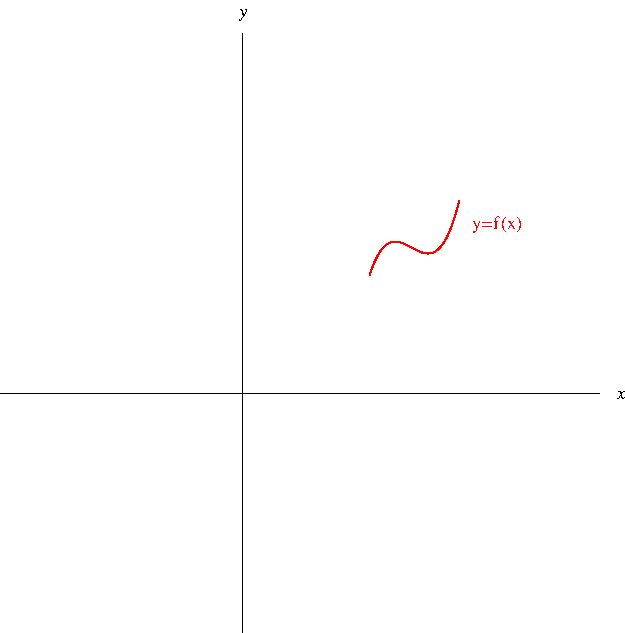
\includegraphics[height=5cm]{precalculus/pictures/01-03-maga.pdf}%
%}%
%\only<handout:0| 3>{%
%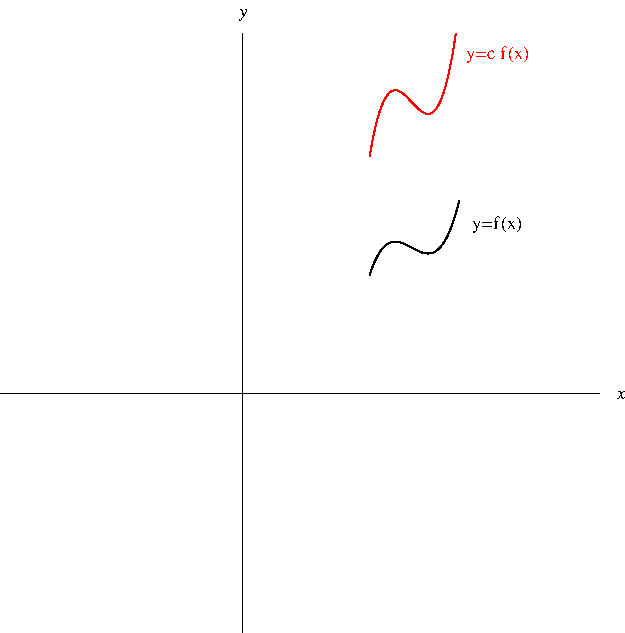
\includegraphics[height=5cm]{precalculus/pictures/01-03-magb.pdf}%
%}%
%\only<handout:0| 4>{%
%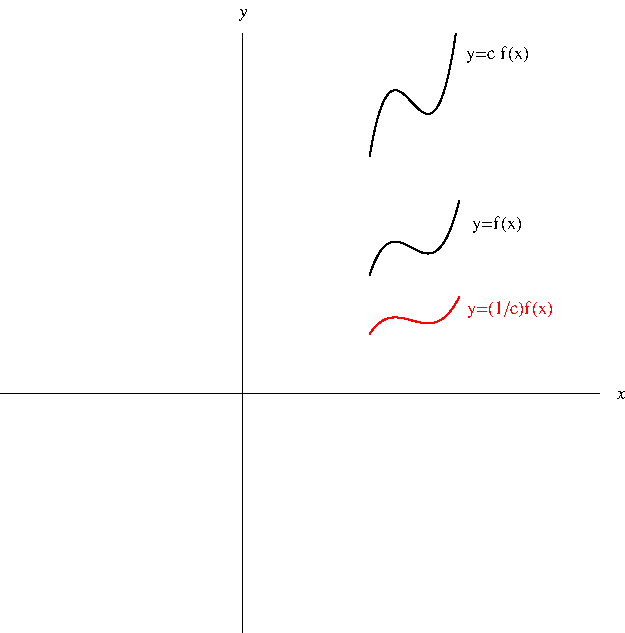
\includegraphics[height=5cm]{precalculus/pictures/01-03-magc.pdf}%
%}%
%\only<handout:0| 5>{%
%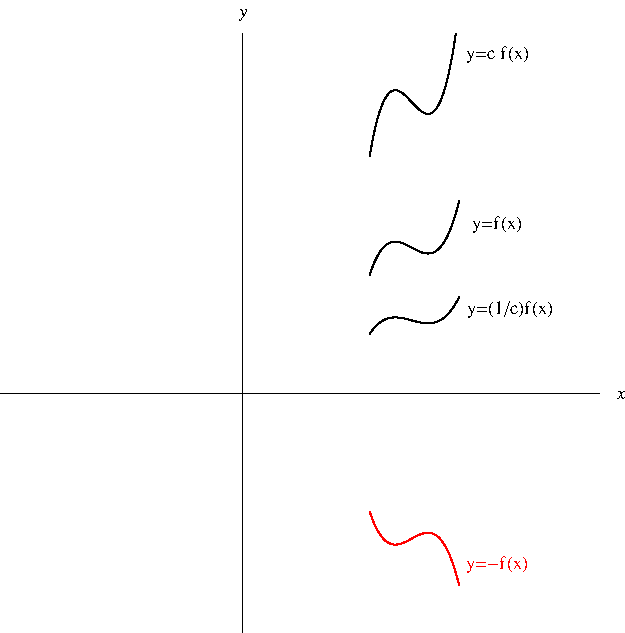
\includegraphics[height=5cm]{precalculus/pictures/01-03-magd.pdf}%
%}%
%\only<6>{%
%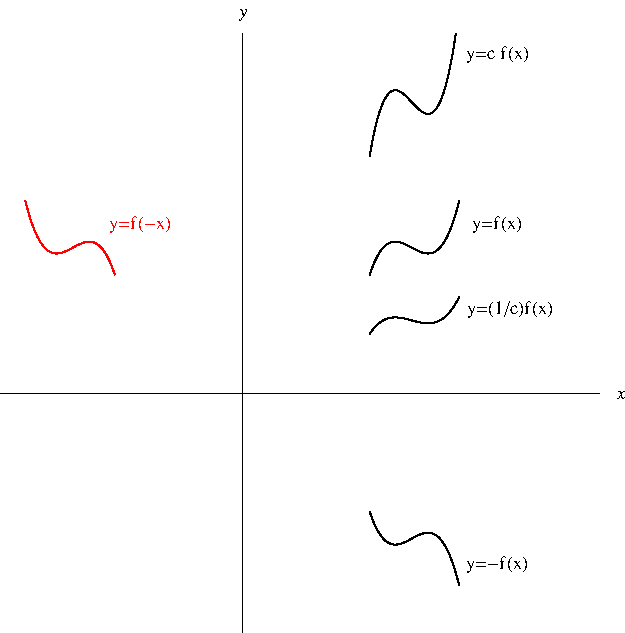
\includegraphics[height=5cm]{precalculus/pictures/01-03-mage.pdf}%
%}%

\column{.5\textwidth}
\alertNoH{3-4}{What happens if we multiply or divide by a constant $c > 1$ in the equation of a function $f$?}  \alertNoH{5}{What happens if we multiply $f$ by $-1$?}  \alertNoH{6}{What happens if we multiply $x$ by $-1$ before applying $f$?}
\end{columns}

\begin{tabular}{|l|l|}
\hline
\alert<handout:0| 3>{$cf(x)$} &%
\uncover<3->{\alert<handout:0| 3>{Stretch the graph of $f(x)$ vertically by a factor of $c$.}} \\%
\alert<handout:0| 4>{$(1/c)f(x)$} &%
\uncover<4->{\alert<handout:0| 4>{Compress the graph of $f(x)$ vertically by a factor of $c$.}} \\%
\alert<handout:0| 5>{$-f(x)$} &%
\uncover<5->{\alert<handout:0| 5>{Reflect the graph of $f(x)$ in the $x$-axis.}} \\%
\alert<handout:0| 6>{$f(-x)$} &%
\uncover<6->{\alert<handout:0| 6>{Reflect the graph of $f(x)$ in the $y$-axis.}}\\%
\hline
\end{tabular}
\uncover<7>{~} %this line is needed to avoid a latexing bug: without this line, the next slide will be messed up.

\end{frame}
% end module transformations-magnifications
